\documentclass[conference]{IEEEtran}
\IEEEoverridecommandlockouts

\usepackage{cite}
\usepackage{amsmath,amssymb,amsfonts}
\usepackage{graphicx}
\usepackage{textcomp}
\usepackage{xcolor}
\usepackage{url}
\usepackage{booktabs}

\graphicspath{{./}{./figures/}}
\DeclareGraphicsExtensions{.pdf,.png,.jpg,.jpeg}

\begin{document}

\title{Spam Message Classification Using Naive Bayes and Logistic Regression}

\author{
\IEEEauthorblockN{Kevin Kayasit Lendvay}
\IEEEauthorblockA{
\textit{Eötvös Loránd University}\\
Budapest, Hungary \\
ajz5ct@inf.elte.hu}
\and
\IEEEauthorblockN{Olivér Révész}
\IEEEauthorblockA{
\textit{Eötvös Loránd University}\\
Budapest, Hungary \\
vg89c7@inf.elte.hu}
}

\maketitle

\begin{abstract}
Short Message Service (SMS) spam filtering remains challenging due to strict
160-character payload limits, informal abbreviations, and severe class
imbalance. This paper benchmarks generative Multinomial Naive Bayes (MNB) and
discriminative $L_2$-regularized Logistic Regression (LR) over sublinear
TF-IDF unigram and bigram features on the UCI SMS Spam Collection
($N = 5574$). Evaluated on a stratified hold-out test set ($N = 1394$), LR
achieves $0.9775$ Average Precision, $94.1\%$ $F_1$-score, and a $0.08\%$
false positive rate, outperforming MNB ($0.9732$ AP, $93.3\%$ $F_1$, $0.25\%$
FPR) while maintaining better probability calibration.
\end{abstract}

\begin{IEEEkeywords}
SMS spam filtering, Multinomial Naive Bayes, Logistic Regression, TF-IDF,
class imbalance, Precision-Recall
\end{IEEEkeywords}


\section{Introduction}

Mobile text messaging is one of the most widely used communication channels
worldwide, making Short Message Service (SMS) a prime target for unsolicited
commercial advertisements, phishing lures, and financial fraud
\cite{10.1145/2034691.2034742, ALMEIDA201625}. Unlike email spam
filtering---where classifiers can inspect routing headers, HTML markup, and
hundreds of tokens per document \cite{metsis2006spam}---content-based SMS
spam filters operate under tight structural constraints. Standard SMS
messages are capped at 140 bytes (160 seven-bit ASCII characters), resulting
in very few words per message and extreme feature sparsity
\cite{10.1145/2034691.2034742}. Moreover, mobile text is rife with phonetic
slang, abbreviations, and deliberate character substitutions (such as
``txt'', ``gr8'', or ``150p'') that degrade standard lexical tokenizers
\cite{ALMEIDA201625}.

\begin{figure*}[!t]
    \centering
    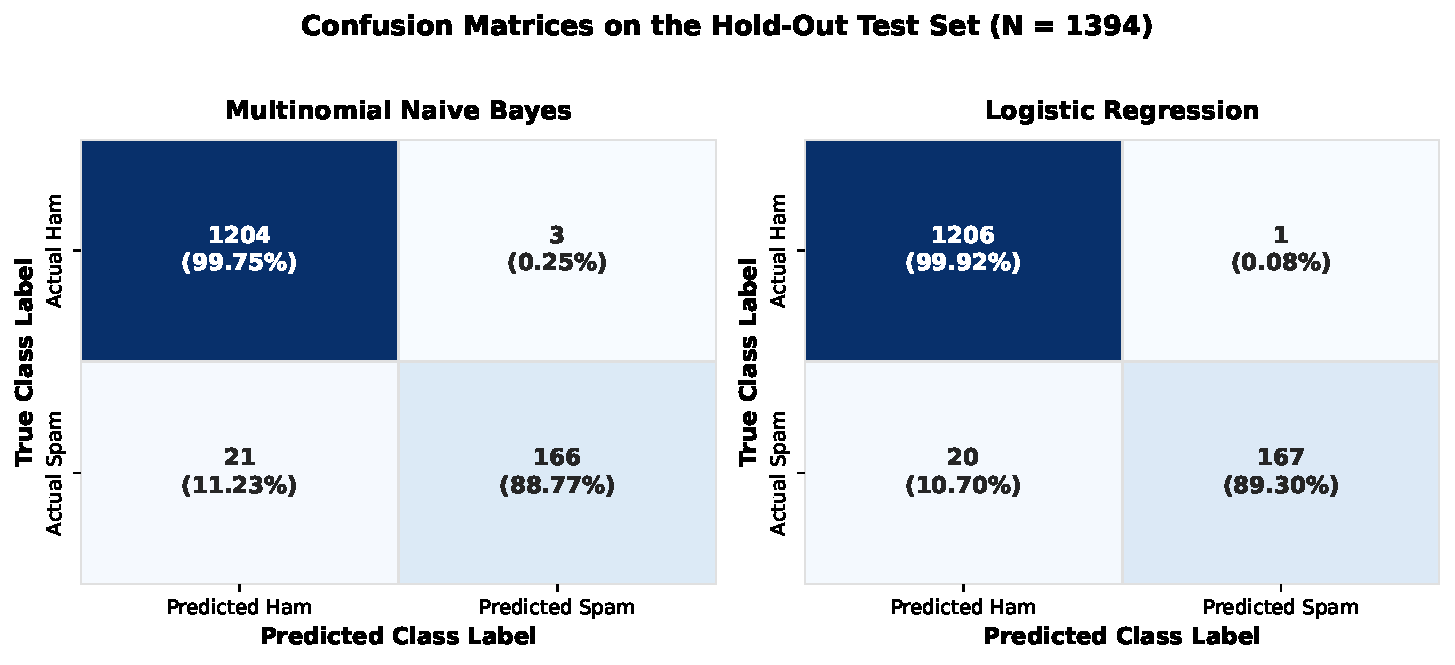
\includegraphics[width=0.76\textwidth]{fig2_confusion_matrices}
    \caption{Confusion matrices on the hold-out test set ($N = 1394$) at the
    default threshold $\tau = 0.50$. Logistic Regression yields only a single
    false positive ($0.08\%$ FPR) compared to $3$ false positives ($0.25\%$
    FPR) for Multinomial Naive Bayes.}
    \label{fig:confusion}
\end{figure*}

From an operational standpoint, SMS spam filtering is governed by an
asymmetric cost structure: a filter must maximize spam detection recall while
keeping the false positive rate (FPR) as close to zero as possible
\cite{10.1145/2034691.2034742, metsis2006spam}. Blocking a legitimate
personal or emergency message (\textit{ham}) is far more disruptive to a user
than letting an occasional advertisement reach the inbox \cite{ALMEIDA201625}.
This trade-off is compounded by the skewed class distribution of real-world
messaging traffic, where spam typically accounts for less than $15\%$ of
volume \cite{10.1145/2034691.2034742, sms_spam_collection_228}. As shown by
Davis and Goadrich \cite{10.1145/1143844.1143874}, Receiver Operating
Characteristic (ROC) curves can present an overly optimistic view on skewed
datasets because the large number of true negatives dominates the FPR
denominator. Rigorous evaluation therefore requires Precision-Recall (PR)
curves alongside explicit threshold sensitivity analysis
\cite{10.1145/1143844.1143874, DREISEITL2002352}.

In this paper, we present a reproducible empirical study comparing classical
generative and discriminative linear classifiers---Multinomial Naive Bayes
(MNB) and $L_2$-regularized Logistic Regression (LR)---on the public UCI SMS
Spam Collection \cite{10.1145/2034691.2034742, sms_spam_collection_228}. Our
main contributions are threefold:
\begin{enumerate}
    \item We formulate and compare Multinomial Naive Bayes
    \cite{mccallum1998comparison, metsis2006spam} and $L_2$-regularized
    Logistic Regression \cite{NIPS2001_7b7a53e2, DREISEITL2002352} over
    sublinear TF-IDF unigram and bigram representations
    \cite{zhang2011comparative}.
    \item We evaluate white-box feature interpretability by contrasting
    learned LR regression weights ($\beta_j$) with MNB log-likelihood ratios
    across the most informative spam tokens.
    \item We analyze probability calibration and operational deployment by
    mapping precision, recall, and false positive rates across decision
    thresholds $\tau \in [0.05, 0.95]$.
\end{enumerate}

\begin{figure}[!t]
    \centering
    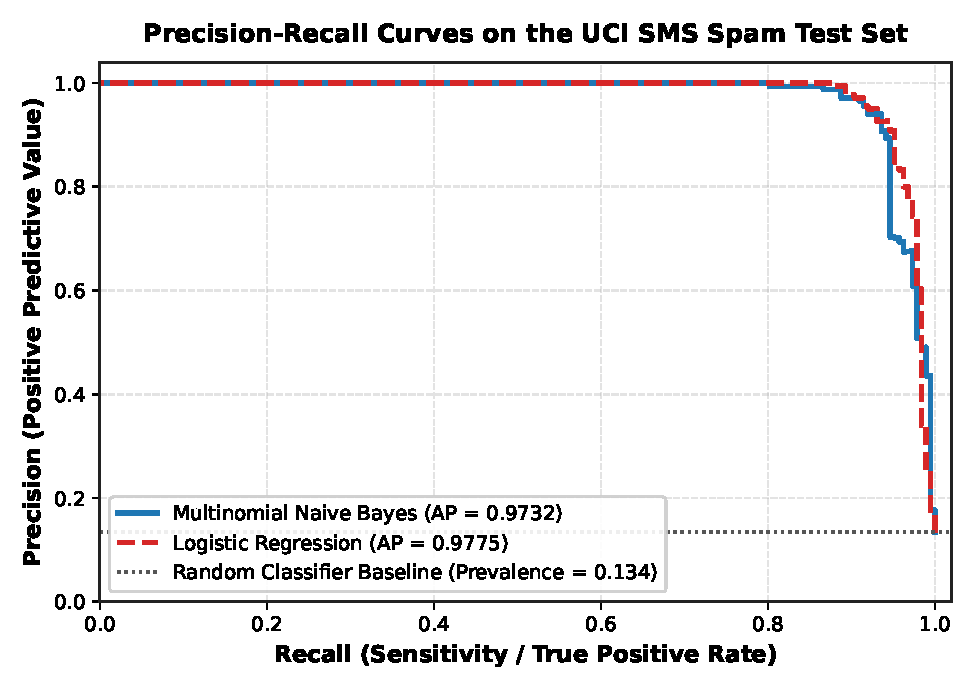
\includegraphics[width=1.0\columnwidth]{fig1_precision_recall_curve}
    \caption{Precision-Recall curves on the UCI SMS Spam hold-out test set
    ($N = 1394$). $L_2$-regularized Logistic Regression achieves a higher
    Average Precision ($\text{AP} = 0.9775$) than Multinomial Naive Bayes
    ($\text{AP} = 0.9732$).}
    \label{fig:pr_curve}
\end{figure}


\section{Related Work}

\subsection{SMS and Email Spam Filtering}
Statistical spam filtering was first studied extensively in electronic mail.
Metsis et al. \cite{metsis2006spam} evaluated five Naive Bayes variants
across six Enron-Spam corpora, showing that Multinomial Naive Bayes and
Flexible Bayes achieve strong cost-sensitive performance when false positives
are heavily penalized. Extending these methods to mobile messaging, Almeida
et al. \cite{10.1145/2034691.2034742} introduced the UCI SMS Spam Collection
\cite{sms_spam_collection_228} and benchmarked 14 classifiers, including
Support Vector Machines (SVM), $k$-Nearest Neighbors ($k$-NN), C4.5 decision
trees, and Naive Bayes variants. Because email filters degrade on short,
noisy texts, Almeida et al. \cite{ALMEIDA201625} later combined lexicographic
normalization (using Lingo and English dictionaries) with semantic concept
expansion from BabelNet to resolve out-of-vocabulary slang, polysemy, and
synonymy in SMS and instant messaging spam.

\begin{figure*}[!t]
    \centering
    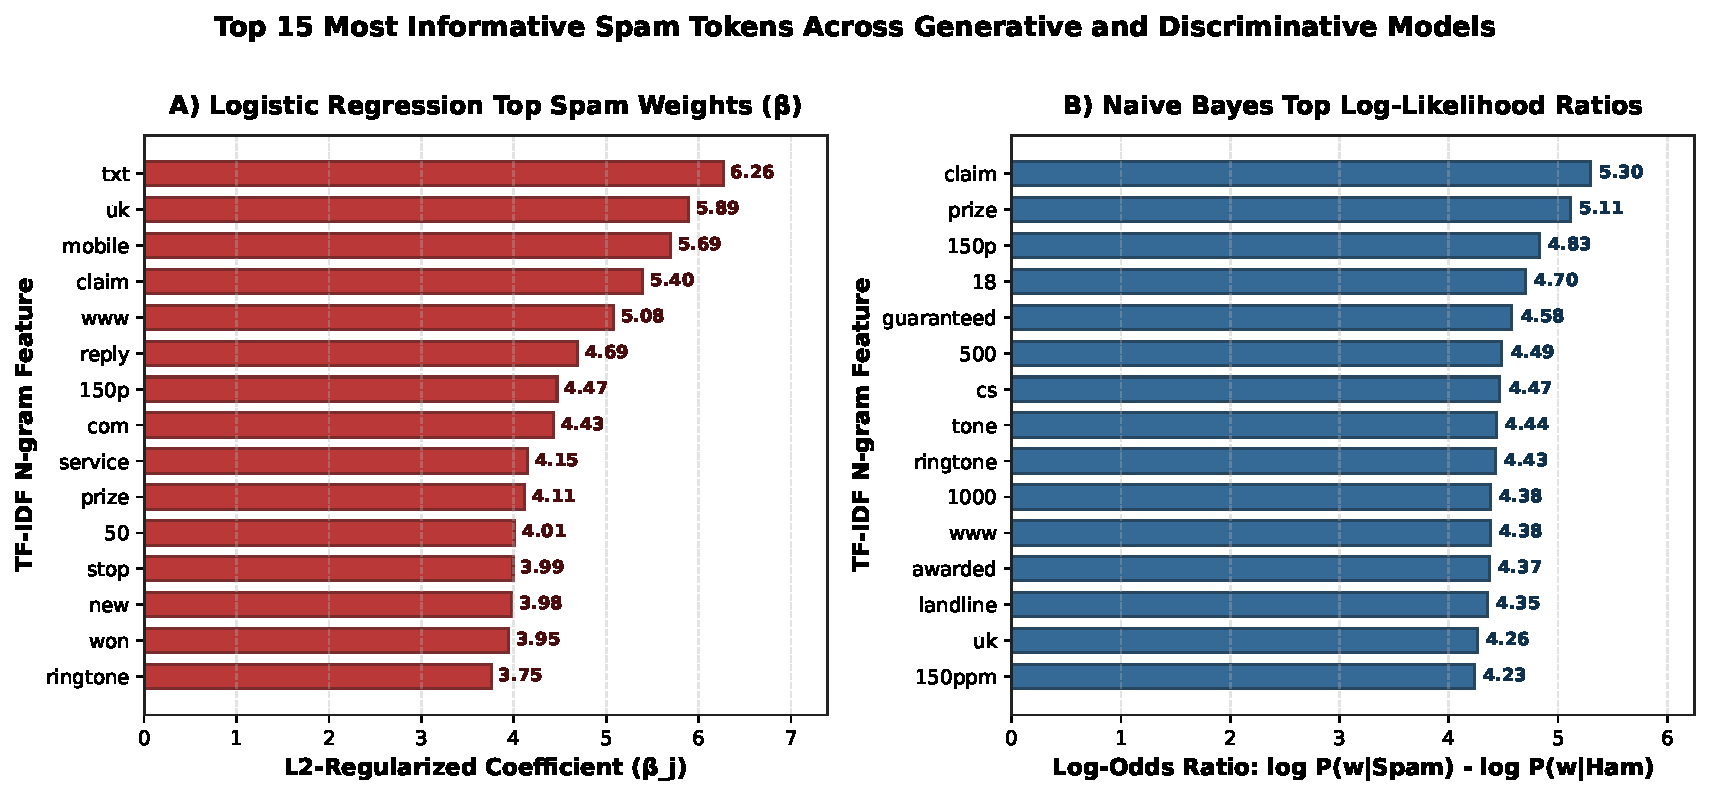
\includegraphics[width=0.78\textwidth]{fig3_top_spam_features}
    \caption{Top 15 most informative spam tokens across (A) $L_2$-regularized
    Logistic Regression weights ($\beta_j$) and (B) Multinomial Naive Bayes
    log-likelihood ratios.}
    \label{fig:features}
\end{figure*}

\subsection{Generative vs. Discriminative Text Categorization}
McCallum and Nigam \cite{mccallum1998comparison} clarified the distinction
between the multi-variate Bernoulli event model (binary word presence) and
the multinomial event model (word frequency counts), demonstrating that the
multinomial formulation reduces classification error by $27\%$ on average
across text corpora. Despite its conditional independence assumption, Naive
Bayes competes well with complex classifiers because zero-one classification
accuracy remains optimal as long as the estimated posterior agrees with the
true distribution on the argmax class, or when feature dependencies cancel
out \cite{zhang2004optimality}.

Comparing generative Naive Bayes and discriminative Logistic Regression, Ng
and Jordan \cite{NIPS2001_7b7a53e2} proved that while discriminative learning
achieves a lower asymptotic error floor, generative Naive Bayes converges
toward its asymptotic error at an $\mathcal{O}(\log n)$ rate rather than
$\mathcal{O}(n)$. Dreiseitl and Ohno-Machado \cite{DREISEITL2002352}
emphasized that Logistic Regression acts as a parametric white-box model
whose coefficients directly measure feature importance, while weight decay
($L_2$ shrinkage) smooths the decision boundary to prevent overfitting.
Furthermore, Zhang et al. \cite{zhang2011comparative} showed that combining
TF-IDF weighting with multi-word sequences captures local context while
retaining strong statistical discriminative power in high-dimensional spaces.


\section{Data}

We use the benchmark UCI SMS Spam Collection
\cite{10.1145/2034691.2034742, sms_spam_collection_228}, which comprises
$5574$ English SMS messages compiled from four sources: $425$ spam messages
from the UK Grumbletext forum, $3375$ ham messages from the NUS SMS Corpus,
$450$ ham messages from Tagg's doctoral thesis, and $1324$ messages ($1002$
ham, $322$ spam) from the SMS Spam Corpus v.0.1 Big
\cite{10.1145/2034691.2034742}. Overall, the dataset contains $4827$
legitimate (\textit{ham}, $86.60\%$) and $747$ unsolicited (\textit{spam},
$13.40\%$) messages. Spam messages average $23.48$ tokens ($17\,543$ tokens
total), whereas ham messages average $13.18$ tokens ($63\,632$ tokens total)
\cite{10.1145/2034691.2034742}.

To preserve the $13.40\%$ spam prior and obtain an unbiased generalization
error estimate \cite{DREISEITL2002352}, we apply a stratified $75\%/25\%$
train--test split, yielding $N_{\text{train}} = 4180$ training messages
($3620$ ham, $560$ spam) and a hold-out test set of $N_{\text{test}} = 1394$
messages ($1207$ ham, $187$ spam). Following Almeida et al.
\cite{10.1145/2034691.2034742}, we omit stop-word removal and stemming so as
not to erase informative triggers. Messages are lowercased and tokenized via
a regular expression pattern that preserves alphanumeric strings, monetary
rates (``150p'', ``150ppm''), numbers (``18'', ``500'', ``1000''), and domain
fragments (``www'', ``uk'', ``com'') while splitting on punctuation
\cite{10.1145/2034691.2034742}. To capture both individual words and
multi-word phrases \cite{zhang2011comparative}, we extract unigrams and
bigrams ($n \in \{1, 2\}$) with minimum document frequency $\text{df} \ge 2$.


\section{Methods}

\subsection{TF-IDF Feature Representation}
Each SMS message $d$ is mapped into a vector $\mathbf{x} \in \mathbb{R}^{V}$
using sublinear Term Frequency--Inverse Document Frequency (TF-IDF) weighting
\cite{zhang2011comparative}:
\begin{equation}
    w_{t,d} = \left(1 + \log \text{tf}(t, d)\right) \cdot
    \left(\log \frac{1 + N_{\text{train}}}{1 + \text{df}(t)} + 1\right),
\end{equation}
where $\text{tf}(t,d)$ is the frequency of term $t$ in $d$ and $\text{df}(t)$
is its training document frequency. Because spam messages are nearly twice as
long as ham messages on average \cite{10.1145/2034691.2034742}, vectors are
$L_2$-normalized ($\tilde{\mathbf{x}} = \mathbf{x} / \|\mathbf{x}\|_2$) to
eliminate length bias \cite{metsis2006spam}.

\subsection{Multinomial Naive Bayes (MNB)}
Under the multinomial event model \cite{mccallum1998comparison,
metsis2006spam}, the posterior log-odds between spam ($y=1$) and ham ($y=0$)
is a linear function of $\tilde{\mathbf{x}}$ \cite{NIPS2001_7b7a53e2}:
\begin{equation}
    \log \frac{P(y=1 \mid \tilde{\mathbf{x}})}{P(y=0 \mid \tilde{\mathbf{x}})}
    = \log \frac{\hat{\pi}_1}{\hat{\pi}_0} +
    \sum_{j=1}^{V} \tilde{x}_j \log \frac{\hat{\theta}_{j \mid 1}}{\hat{\theta}_{j \mid 0}},
\end{equation}
where $\hat{\pi}_c = N_c / N_{\text{train}}$ is the empirical class prior and
$\hat{\theta}_{j \mid c}$ is estimated via Laplace smoothing ($\alpha > 0$)
\cite{mccallum1998comparison, metsis2006spam}:
\begin{equation}
    \hat{\theta}_{j \mid c} =
    \frac{\sum_{i: y^{(i)}=c} \tilde{x}_j^{(i)} + \alpha}
    {\sum_{k=1}^{V} \sum_{i: y^{(i)}=c} \tilde{x}_k^{(i)} + \alpha V}.
\end{equation}
Token importance in MNB is quantified by the log-likelihood ratio
$\text{LLR}(t_j) = \log \hat{\theta}_{j \mid 1} - \log \hat{\theta}_{j \mid 0}$.

\subsection{Discriminative $L_2$-Regularized Logistic Regression}
Logistic Regression directly models the posterior
$P(y=1 \mid \tilde{\mathbf{x}}) = \sigma(\boldsymbol{\beta}^\top \tilde{\mathbf{x}} + b)$
via the logistic sigmoid $\sigma(z) = (1 + e^{-z})^{-1}$
\cite{NIPS2001_7b7a53e2, DREISEITL2002352}. Parameters $(\boldsymbol{\beta}, b)$
are learned by minimizing the $L_2$-penalized binary cross-entropy loss
\cite{DREISEITL2002352}:
\begin{equation}
    \mathcal{L}(\boldsymbol{\beta}, b) =
    -\sum_{i=1}^{N_{\text{train}}} \left[ y^{(i)} \log p_i +
    (1 - y^{(i)}) \log (1 - p_i) \right] +
    \frac{\lambda}{2} \|\boldsymbol{\beta}\|_2^2,
\end{equation}
where $p_i = \sigma(\boldsymbol{\beta}^\top \tilde{\mathbf{x}}^{(i)} + b)$ and
$\lambda > 0$ controls weight shrinkage, smoothing the decision boundary to
prevent overfitting on correlated $n$-grams \cite{DREISEITL2002352}.

\begin{table}[!t]
\centering
\caption{Classification Performance on the Hold-Out Test Set ($N = 1394$)}
\label{tab:results}
\setlength{\tabcolsep}{3.5pt}
\begin{tabular}{lcccccc}
\toprule
\textbf{Model} & \textbf{Prec. (\%)} & \textbf{Rec. (\%)} & \textbf{$\text{F}_1$ (\%)} & \textbf{FPR (\%)} & \textbf{AP} \\
\midrule
Multinomial NB      & 98.22 & 88.77 & 93.26 & 0.25 & 0.9732 \\
Logistic Regression & \textbf{99.40} & \textbf{89.30} & \textbf{94.08} & \textbf{0.08} & \textbf{0.9775}\\
\bottomrule
\end{tabular}
\end{table}

\begin{figure*}[!t]
    \centering
    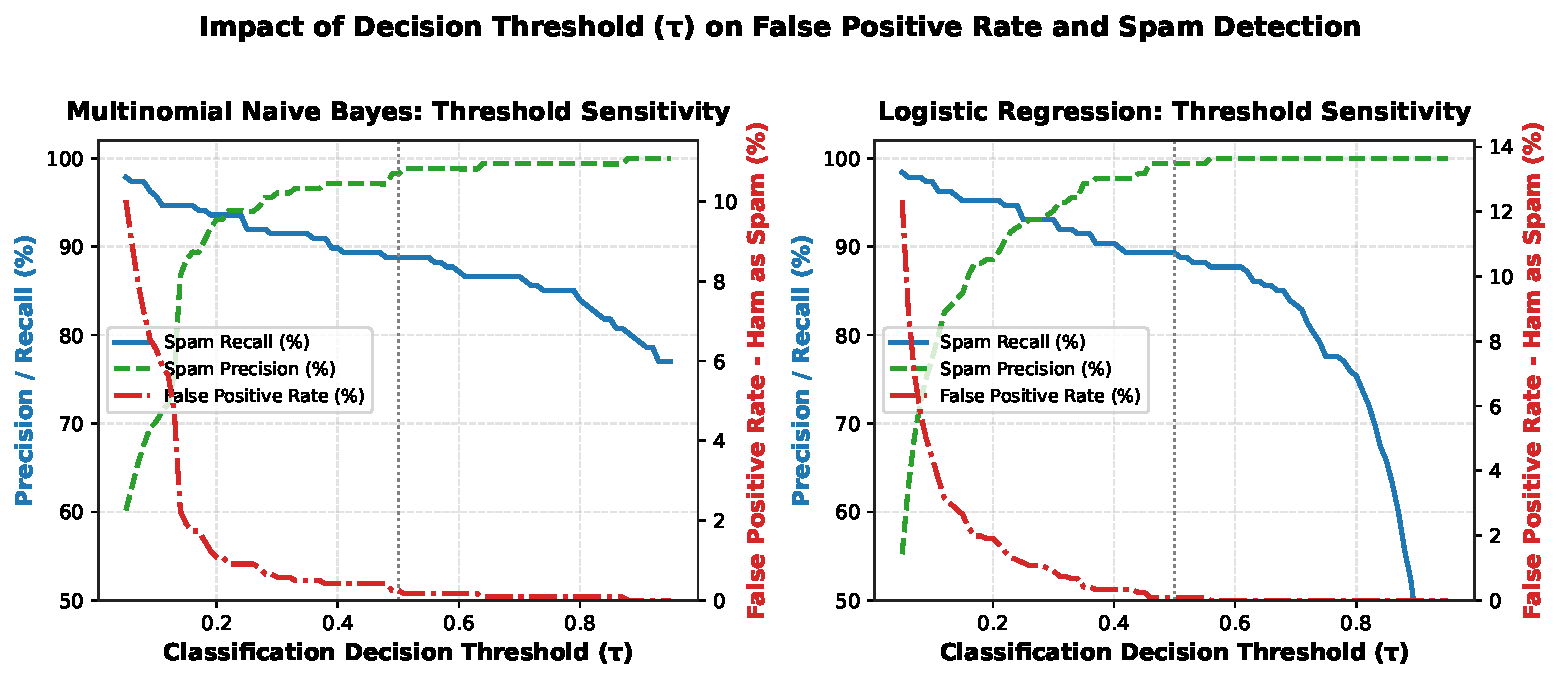
\includegraphics[width=0.78\textwidth]{fig4_threshold_fpr_tradeoff}
    \caption{Impact of classification decision threshold ($\tau$) on Spam
    Precision, Recall, and False Positive Rate (FPR) for Multinomial Naive
    Bayes and Logistic Regression.}
    \label{fig:threshold}
\end{figure*}


\section{Results and Discussion}

\subsection{Precision-Recall and Confusion Matrix Evaluation}
Given the skewed test distribution ($1207$ ham vs. $187$ spam messages,
$13.4\%$ prevalence), we evaluate classifiers in Precision-Recall space
\cite{10.1145/1143844.1143874}. Fig.~\ref{fig:pr_curve} shows the PR curves
for MNB and LR, and Table~\ref{tab:results} summarizes all metrics. Both
linear classifiers maintain nearly $100\%$ precision up to $80\%$ recall.
Across the full recall range, $L_2$-regularized Logistic Regression achieves
$\text{AP} = 0.9775$, outperforming Multinomial Naive Bayes
($\text{AP} = 0.9732$). Consistent with Ng and Jordan \cite{NIPS2001_7b7a53e2},
at $N_{\text{train}} = 4180$, discriminative training reaches its lower
asymptotic error regime, whereas MNB is slightly degraded by correlated
unigrams and bigrams. Both models train in milliseconds ($0.002\text{ s}$ for
MNB and $0.015\text{ s}$ for LR).

At the default threshold $\tau = 0.50$ (Fig.~\ref{fig:confusion}), MNB
misclassifies $3$ of $1207$ ham messages ($\text{TN} = 1204$, $\text{FP} = 3$,
$\text{FPR} = 0.25\%$) and detects $166$ of $187$ spam messages
($\text{TP} = 166$, $\text{FN} = 21$, $\text{Recall} = 88.77\%$), yielding
$98.22\%$ precision and $93.26\%$ $F_1$. Logistic Regression cuts false
positives to a single message ($\text{TN} = 1206$, $\text{FP} = 1$,
$\text{FPR} = 0.08\%$) while catching $167$ spam messages ($\text{TP} = 167$,
$\text{FN} = 20$, $\text{Recall} = 89.30\%$), achieving $99.40\%$ precision
and $94.08\%$ $F_1$. Both models improve substantially upon the unigram
baselines in Almeida et al. \cite{10.1145/2034691.2034742} (where linear SVM
caught $83.10\%$ of spam at $0.18\%$ FPR, and MNB caught $52.06\%$).

\subsection{Feature Interpretability: Generative vs. Discriminative}
Inspecting white-box model parameters \cite{DREISEITL2002352} in
Fig.~\ref{fig:features} reveals how LR weights $\beta_j$ (Panel A) and MNB
log-odds ratios (Panel B) rank the top 15 spam tokens. Both models highlight
commercial triggers such as \texttt{claim} ($\beta = 5.40$,
$\text{LLR} = 5.30$), \texttt{prize} ($\beta = 4.11$, $\text{LLR} = 5.11$),
\texttt{150p} ($\beta = 4.47$, $\text{LLR} = 4.83$), \texttt{www}
($\beta = 5.08$, $\text{LLR} = 4.38$), \texttt{uk} ($\beta = 5.89$,
$\text{LLR} = 4.26$), and \texttt{ringtone} ($\beta = 3.75$,
$\text{LLR} = 4.43$).

However, because MNB estimates conditional probabilities independently
\cite{mccallum1998comparison, zhang2004optimality}, its top log-odds ratios
favor narrow, campaign-specific tokens that rarely occur in ham (\texttt{18}
$\text{LLR} = 4.70$, \texttt{guaranteed} $\text{LLR} = 4.58$, \texttt{500}
$\text{LLR} = 4.49$, \texttt{1000} $\text{LLR} = 4.38$, \texttt{150ppm}
$\text{LLR} = 4.23$). Conversely, joint optimization under $L_2$ shrinkage
\cite{DREISEITL2002352} leads LR to assign its largest weights to broad
call-to-action tokens (\texttt{txt} $\beta = 6.26$, \texttt{uk}
$\beta = 5.89$, \texttt{mobile} $\beta = 5.69$, \texttt{reply}
$\beta = 4.69$, \texttt{service} $\beta = 4.15$, \texttt{stop}
$\beta = 3.99$), avoiding redundant double-counting.

\subsection{Decision Threshold Sensitivity and Calibration}
To assess probability calibration across operating points
\cite{DREISEITL2002352, metsis2006spam}, Fig.~\ref{fig:threshold} plots
precision, recall, and FPR across $\tau \in [0.05, 0.95]$. Below
$\tau = 0.20$, both models achieve $>95\%$ recall but suffer from excessive
false positive rates ($10\%$--$13\%$). Above $\tau = 0.25$, FPR drops below
$1\%$. Because MNB multiplies correlated token likelihoods, its posteriors
are pushed toward $0$ and $1$ \cite{metsis2006spam, zhang2004optimality},
resulting in a gradual recall decay from $88.8\%$ at $\tau = 0.50$ to $77.0\%$
at $\tau = 0.95$. In contrast, LR exhibits a well-calibrated plateau across
$\tau \in [0.45, 0.65]$, maintaining $99.4\%$--$100\%$ precision and
$\approx 88\%$--$89.3\%$ recall at $\le 0.08\%$ FPR, confirming $\tau = 0.50$
as a robust operating threshold.


\section{Conclusion}

We replicated and compared Multinomial Naive Bayes and $L_2$-regularized
Logistic Regression on the UCI SMS Spam Collection
\cite{10.1145/2034691.2034742, sms_spam_collection_228}. Coupling sublinear
TF-IDF unigram and bigram features with $L_2$-regularized Logistic Regression
achieves $99.40\%$ precision, $94.08\%$ $F_1$-score, $\text{AP} = 0.9775$,
and a $0.08\%$ FPR in just $15\text{ ms}$ of training time, outperforming
Multinomial Naive Bayes in both discriminative accuracy and probability
calibration.

\bibliographystyle{IEEEtran}
\bibliography{references}

\end{document}